\documentclass[12pt]{article}
\usepackage[portuguese]{babel}
\usepackage[utf8]{inputenc}
\usepackage{graphicx}
\usepackage[pdfborder={0 0 0}]{hyperref}
\usepackage{fancyhdr}
\usepackage{textcomp}

\author{}
\usepackage[T1]{fontenc}
\usepackage[utf8]{luainputenc}
\usepackage{geometry}
\usepackage{imakeidx}
\usepackage{indentfirst}
\usepackage{titlesec}
\usepackage{longtable}
\usepackage{verbatim}
\usepackage{amsmath}

\usepackage[portuguese]{babel}
%\usepackage[utf8]{inputenc}
\usepackage{graphicx}

\setcounter{secnumdepth}{4}

\geometry{verbose,margin=2cm}
\setlength{\parindent}{0cm}
\PassOptionsToPackage{normalem}{ulem}
\usepackage{ulem}
\linespread{1.5}
\usepackage{graphicx}
\makeatletter
%%%%%%%%%%%%%%%%%%%%%%%%%%%%%% User specified LaTeX commands.
\date{}

\newcommand*{\plogo}{\fbox{$\mathcal{ESIDEI-RG}$}}

\newcommand{\HRule}{\rule{\linewidth}{0.5mm}}
\newcommand*\sepline{%
	\begin{center}
		\rule[1ex]{\textwidth}{.5pt}
	\end{center}}
\newcommand{\itab}[1]{\hspace{-0.05\textwidth}\rlap{#1}}
\newcommand{\tab}[2]{\typeout{#2} \hspace{#2 \textwidth}\rlap{#1}}
\newcommand{\listAuthor}[5]
{
	\itab{#1,} \tab{\textsc{#2}}{.15} \tab{\texttt{#3}}{.12} \tab{#4}{.42} \tab{#5}{.175}\\
}

\errorcontextlines 10000

\begin{document}
%\pagestyle{firststyle}
\begin{titlepage}
%\thispagestyle{firststyle}
\begin{center}
\textsc{\LARGE Departamento de Engenharia Informática}\\[1.5cm]
\sepline
{ \huge \bfseries Compiladores}\\[0.4cm]
\textsc{\LARGE 01/06/2015}
\sepline

{\huge \bfseries Compilador para a linguagem mili-Pascal (mPa)}\\[0.4cm]

\textbf{Mooshak Login: Migueis}

\sepline
\listAuthor{Quitério}{Pedro}{pmlour@student.dei.uc.pt}{2012143635}{LEI}
\listAuthor{Subtil}{João}{jsubtil@student.dei.uc.pt}{2012151975}{LEI}

\sepline

\end{center}
\end{titlepage}

\newpage

\pagestyle{fancy}
\fancyhf{}
\rhead{Migueis}
\lhead{Compiladores - MiliPascal - \leftmark}
\rfoot{Página \thepage}
\lfoot{Junho 2015}




\tableofcontents
%\printindex
\newpage

%%%%%%%%%%%%%%%%%%%%%%%%%%%%%%%%%%%%%%%%%%%%%%%%%%%%%%%%%%%%%%%%%%%%%%%%%%%%%%%%%%%%%%%%%%%%%%%%%%%%%%%%%%%

\section{Introdução}

\setlength{\parindent}{1cm} No presente trabalho pretende-se desenvolver um compilador para a linguagem mili-Pascal, um pequeno subconjunto da Linguagem Pascal. Devido ao facto de se tratar de um subconjunto de Pascal, qualquer linguagem aceite por mili-Pascal será também aceite pela linguagem Pascal, podendo, no entanto, não se verificar o contrário.\\
\indent O projecto foi estruturado em 4 fases:
\begin{enumerate}

\item Análise lexical, na qual se recorreu à ferramenta \textbf{Lex};
\item Análise sintática, tendo-se recorrido à ferramenta \textbf{yacc};
\item Construção de tabelas de símbolos e detecção de erros semânticos;
\item Geração de código em LLVM;

\end{enumerate}

\indent 

\noindent O seginte esquema ilustra as fases de compilação:

\begin{center}
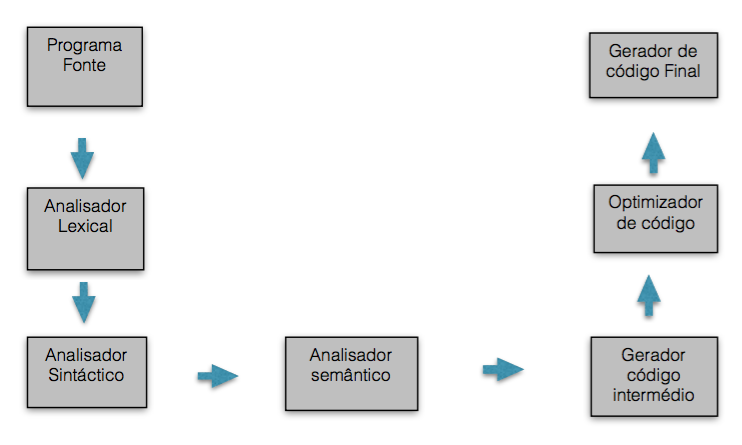
\includegraphics[scale=.7]{fases_de_compilacao.png}\\
Fig.1 - Fases de Compilação;
\end{center}

\newpage

%%%%%%%%%%%%%%%%%%%%%%%%%%%%%%%%%%%%%%%%%%%%%%%%%%%%%%%%%%%%%%%%%%%%%%%%%%%%%%%%%%%%%%%%%%%%%%%%%%%%%%%%%%%

\section{Análise Lexical}
\indent A análise lexical consiste em analisar o \textit{input} introduzido e, a partir do mesmo, produzir uma cadeia de símbolos (\textit{tokens}) que possam ser manipulados pelo \textit{parser}.\\
\indent 
\indent No nosso analisador os comentários são tratados com recurso a uma macro. Assim, sempre que o \textbf{lex} lê (*  *) ou \{ \} ou uma mistura entre os dois, o analisador ignora o que estiver dentro desses caracteres.\\
\indent Sempre que é detectado um caracter ou uma sequência de caracteres que não constituam um token, é gerado um erro lexical, sendo impressa uma mensagem de erro contendo o tipo, linha e coluna de ocorrência (Esta mensagem é diferente, para se distinguir dos restantes tipos de erros que possam existir).

%%%%%%%%%%%%%%%%%%%%%%%%%%%%%%%%%%%%%%%%%%%%%%%%%%%%%%%%%%%%%%%%%%%%%%%%%%%%%%%%%%%%%%%%%%%%%%%%%%%%%%%%%%%

\subsection{Tokens}

\indent De seguida, apresentamos a lista de tokens aceites pela linguagem. Foram também definidos novos tokens para facilitar a construção da AST numa fase posterior.\\

\begin{itemize}

\item \textbf{ID}: Sequências alfanuméricas começadas por uma letra e seguidas por uma combinação de letras e/ou números \textbf{ `` [a-z][a-z0-9]* '' };

\item \textbf{Intlit}: Sequências de dígitos decimais \textbf{ `` [0-9]+ ''};

\item \textbf{Reallit}: Sequências de dígitos decimais interrompidas por um único ponto e opcionalmente seguidas de um exponente, ou sequências de dígitos decimais seguidas de um expoente. O expoente consiste na letra ``e'', opcionalmente seguida de um sinal de + ou de -, seguida de uma sequência de dígitos decimais. \textbf{ `` \{num\}(``.''\{num\})?(e[-+]?\{num\})? '' };

\item \textbf{String}: Sequências de caracteres (excluindo mudanças de linha) iniciadas por uma aspa simples (\textquotesingle) ou terminadas pela primeira ocorrência de uma aspa simples que não seja seguida imediatamente por outra aspa simples. \textbf{\textquotedblleft \textquotesingle \textquotedblright([\^  \space \textbackslash n\textquotesingle]|\textquotesingle\textquotesingle)*\textquotedblleft\textquotesingle\textquotedblright};

\item \textbf{Assign}: \textbf{``:=''};

\item \textbf{Begin}: \textbf{``begin''};

\item \textbf{Colon}: \textbf{``:''};

\item \textbf{Comma}: \textbf{``,''};

\item \textbf{Do}: \textbf{``do''};

\item \textbf{Dot}: \textbf{``.''};

\item \textbf{Else}: \textbf{``else''};

\item \textbf{End}: \textbf{``end''};

\item \textbf{Function}: \textbf{``function''};

\item \textbf{If}: \textbf{``if''};

\item \textbf{Lbrac}: \textbf{``(''};

\item \textbf{Not}: \textbf{``not''};

\item \textbf{Output}: \textbf{``output''};

\item \textbf{Paramstr}: \textbf{``paramstr''};

\item \textbf{Program}: \textbf{``program''};

\item \textbf{Rbrac}: \textbf{``)''};

\item \textbf{Repeat}: \textbf{``repeat''};

\item \textbf{Semic}: \textbf{``;''};

\item \textbf{Then}: \textbf{``then''};

\item \textbf{Until}: \textbf{``until''};

\item \textbf{Val}: \textbf{``val''};

\item \textbf{Var}: \textbf{``var''};

\item \textbf{While}: \textbf{``while''};

\item \textbf{Writeln}: \textbf{``writeln''};

\item \textbf{Op1}: \textbf{``and'' | ``or''};

\item \textbf{Op2}: \textbf{``<'' | ``>'' | ``='' | ``<>'' | ``<='' | ``>=''};

\item \textbf{Op3}: \textbf{``+'' | ``-''};

\item \textbf{Op4}: \textbf{``*'' | ``/'' | ``mod'' | ``div''};

\item \textbf{RESERVED}: palavras reservadas e identificadores requeridos do Pascal standard não usados;

\end{itemize}

\indent Foram criados novos tokens com base na separação dos tokens OP1, OP2 e OP4 para resolver problemas de ambiguidade. As transformações encontram-se apresentadas em baixo:

\begin{itemize}

\item A \textbf{OP1} foi dividida em \textbf{AND} e \textbf{OR}

\item Em \textbf{OP2} \textbf{``<>''} passou a \textbf{NEQ}, \textbf{``<=''} passou a \textbf{LEQ}, \textbf{``>=''} passou a \textbf{GEQ};

\item Na \textbf{OP4} \textbf{``mod''} e \textbf{``div''} passaram a \textbf{MOD} e \textbf{DIV}, respectivamente;

\item \textbf{BEGIN} passou a \textbf{BEG};

\end{itemize}


\newpage

%%%%%%%%%%%%%%%%%%%%%%%%%%%%%%%%%%%%%%%%%%%%%%%%%%%%%%%%%%%%%%%%%%%%%%%%%%%%%%%%%%%%%%%%%%%%%%%%%%%%%%%%%%%

\subsection{Comentários}

\indent Para identificar correctamente os comentários recorremos à macro TESTCOMENT.\\
\indent Quando é detectado o ínicio de um comentário tudo é ignorado até ao caracter de terminação ser detectado.\\
\indent Através desta macro, são também tratados os casos de comentários multi-linha.\\
\indent Dentro de um comentário, todos os caracteres que não servem para fechar o comentário são tratados da mesma forma (apenas é incrementada a coluna), com excepção do caracter de mudança de linha (que incrementa a contagem de linhas e reinicia a contagem de colunas).
\indent Caso seja detectado um \textbf{<<EOF>>} sem o comentário ter sido terminado correctamente, é exibida uma mensagem de erro com a linha e coluna em que começa o mesmo.

\subsection{Tratamento de Erros}

\indent Tal como foi referido anteriormente, sempre que o analisador detecta um erro (comentário/string não terminado(a)) é impressa uma mensagem de erro específica que indica a linha e coluna em que o mesmo ocorreu.\\
\indent Quando é detectado um caracter ilegal (um caracter que não corresponda aos tokens esperados) é impressa a mensagem \textit{``illegal character''} com a respectiva linha e coluna, continuando o programa até ao fim.\\
\indent Após todo o conteúdo ter sido analisado o programa termina e imprime as mensagens correspondentes aos erros detectados, se existirem.

\newpage

\subsection{Linhas e colunas}

\indent Apesar de a contagem de linhas e colunas estar funcional para a primeira e segunda metas, a mesma teve que ser alterada para ficar totalmente funcional para a meta 3, onde esses valores são necessários para a correcta apresentação dos erros semânticos.\\
\indent Deste modo, alterámos o uso de variáveis do tipo \textit{extern} para o uso de uma \textbf{macro} interna do \textbf{lex} que permitiu a passagem correcta dos valores o programa de detecção de erros.

\begin{center}
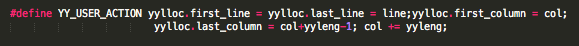
\includegraphics[scale=0.9]{column_line_macro.png}\\
Fig.2 - Macro para contagem de linhas e colunas;
\end{center}


\newpage

\section{Análise Sintáctica}

\indent O analisador sintáctico foi implementado com recurso à ferramenta \textbf{yacc}.\\
\indent A ideia passa por o \textbf{lex} reconhecer os tokens e posteriormente enviá-los ao \textbf{yacc} que irá verificar se a sua organização está de acordo com a estrutura sintática da linguagem.\\
\indent O \textbf{lex} executa a função \textit{yylex()} que trata e envia os tokens para o \textbf{yacc} que corre a partir da função \textit{yyarse()}, produzindo um conjunto de saída (neste caso, uma \textbf{AST}).\\ 
\indent Sempre que o \textbf{lex} identifica um token, envia-o ao \textbf{yacc}. Contudo, este token pode ser recebido como yytext numa estrutura union criada especial para facilitar a manipulação e armazenamento de dados ou pode ser enviado como token que também está definido no início do ficheiro \textit{mpaparser.y}.

\begin{center}
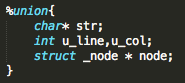
\includegraphics[scale=1]{union_struct.png}\\
Fig.3 - Estrutura Union;
\end{center}

\indent Esta estrutura contém um campo (char*) para armazenar Id\textquotesingle s, Intlit\textquotesingle s, Reallit\textquotesingle s e String\textquotesingle s, um campo para a linha e coluna (embora não estejam a ser usados) e por fim uma estrutura (\textit{\_node}) que depois irá ser utilizada para a construção da AST. \\
\indent Foi necessário também definir algumas variáveis externas como o yytext, linha e coluna para partilhar valores entre ambos os programas.

\begin{center}
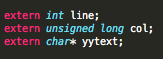
\includegraphics[scale=1]{extern_vars.png}\\
Fig.4 - Variáveis Externas;
\end{center}

\newpage

%%%%%%%%%%%%%%%%%%%%%%%%%%%%%%%%%%%%%%%%%%%%

\subsection{Gramática}

\indent A gramática é a maneira formal de especificar a sintaxe de uma linguagem. Para o projecto foi fornecida a gramática na forma \textbf{EBNF} (\textit{Extended Backus–Naur Form}), tendo esta que ser transformada em \textbf{BNF} (\textit{Backus–Naur Form}) para remover as ambiguidades.

\subsubsection{Gramática inicial}

\noindent Prog $\rightarrow$ ProgHeading SEMIC ProgBlock DOT\\
ProgHeading $\rightarrow$ PROGRAM ID LBRAC OUTPUT RBRAC\\
ProgBlock $\rightarrow$ VarPart FuncPart StatPart\\
VarPart $\rightarrow$ [ VAR VarDeclaration SEMIC \{ VarDeclaration SEMIC \} ]\\
VarDeclaration $\rightarrow$ IDList COLON ID\\
IDList $\rightarrow$ ID \{ COMMA ID \}\\
FuncPart $\rightarrow$ \{ FuncDeclaration SEMIC \}\\
FuncDeclaration $\rightarrow$ FuncHeading SEMIC FORWARD\\
FuncDeclaration $\rightarrow$ FuncIdent SEMIC FuncBlock\\
FuncDeclaration $\rightarrow$ FuncHeading SEMIC FuncBlock\\
FuncHeading $\rightarrow$ FUNCTION ID [ FormalParamList ] COLON ID\\
FuncIdent $\rightarrow$ FUNCTION ID\\
FormalParamList $\rightarrow$ LBRAC FormalParams \{ SEMIC FormalParams \} RBRAC\\
FormalParams $\rightarrow$ [ VAR ] IDList COLON ID\\
FuncBlock $\rightarrow$ VarPart StatPart\\
StatPart $\rightarrow$ CompStat\\
CompStat $\rightarrow$ BEGIN StatList END\\
StatList $\rightarrow$ Stat \{ SEMIC Stat \}\\
Stat $\rightarrow$ CompStat\\
Stat $\rightarrow$ IF Expr THEN Stat [ ELSE Stat ]\\
Stat $\rightarrow$ WHILE Expr DO Stat\\
Stat $\rightarrow$ REPEAT StatList UNTIL Expr\\
Stat $\rightarrow$ VAL LBRAC PARAMSTR LBRAC Expr RBRAC COMMA ID RBRAC\\
Stat $\rightarrow$ [ ID ASSIGN Expr ]\\
Stat $\rightarrow$ WRITELN [ WritelnPList ]\\
WritelnPList $\rightarrow$ LBRAC ( Expr | STRING ) \{ COMMA ( Expr | STRING ) \} RBRAC\\
Expr $\rightarrow$ Expr (OP1 | OP2 | OP3 | OP4) Expr\\
Expr $\rightarrow$ (OP3 | NOT) Expr\\
Expr $\rightarrow$ LBRAC Expr RBRAC\\
Expr $\rightarrow$ INTLIT | REALLIT\\
Expr $\rightarrow$ ID [ ParamList ]\\
ParamList $\rightarrow$ LBRAC Expr \{COMMA Expr\} RBRAC\\

\subsubsection{Gramática na forma BNF}

\noindent Para remover as ambiguidades tivemos de efectuar diversas alterações, tais como:

\begin{itemize} 

\item Criação de estados adicionais para regras que implicam repetição de tokens;

\item Estabelecimente de prioridades entre operadores;

\item Definição de regras de associação;

\end{itemize}

\begin{center}
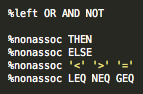
\includegraphics[scale=1]{operators_precedence.png}\\
Fig.4 - Precedência de Operadores;
\end{center}

\newpage

\indent A gramática resultante das operações acima descritas é a seguinte:

\begin{center}
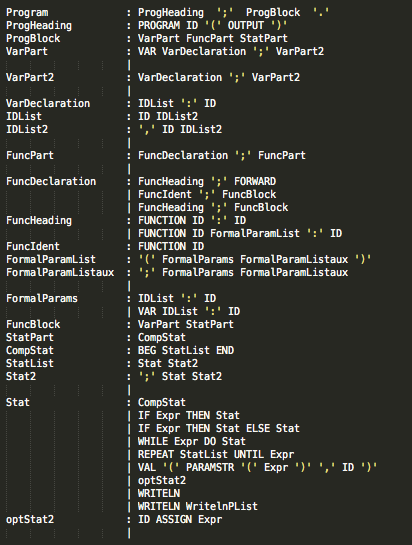
\includegraphics[scale=1]{bnf_grammar_part1.png}\\
Fig.6 - Gramática BNF - parte 1;
\end{center}

\newpage

\begin{center}
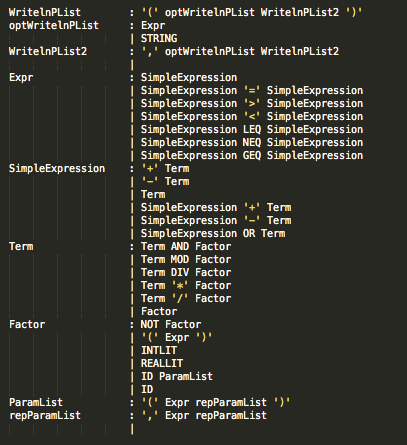
\includegraphics[scale=1]{bnf_grammar_part2.png}\\
Fig.7 - Gramática BNF - parte 2;
\end{center}

\newpage

\subsection{Tratamento de erros sintácticos}

\indent O tratamento de erros sintácticos é feito recorrendo à função \textit{yyerror()} que imprime a linha, coluna e erro detectado.

\begin{center}
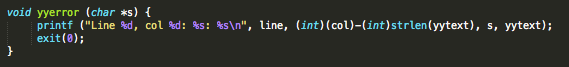
\includegraphics[scale=0.9]{yyerror.png}\\
Fig.8 - Função \textit{yyerror};
\end{center}

\subsection{Árvore de Sintaxe Abstracta - AST}

\indent Para a estrutura da árvore decidimos criar um nó genérico que contém a informação necessária para tornar o seu acesso mais simples tanto na sua criação como em acessos futuros (nomeadamente, durante a criação das tabelas de símbolos e tratamento de erros).\\

\begin{center}
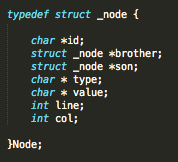
\includegraphics[scale=0.9]{node_struct.png}\\
Fig.9 - Estrutura do nó genérico;
\end{center}

\indent O campo \textit{id} é o nome do respectivo nó com o seu valor entre parênteses e \textit{brother} e \textit{son} são ponteiros para o irmão e o filho respectivamente. Existe ainda \textit{line} e \textit{col} para facilitar a impressão de erros na fase de análise semântica.\\
\indent Os campos \textit{type} e \textit{value} são utilizados para guardar Id\textquotesingle s, Intlit\textquotesingle s, Reallit\textquotesingle s e String\textquotesingle s.\\
\indent Escolhemos criar a estrutura desta forma por ser mais fácil fazer comparações quando necessário. Assim, em vez de ler \textit{``Intlit(\%)''} no id e fazer várias operações sobres essas strings, podemos utilizar directamente um simples \textit{strcmp()} sobre os campos \textit{type} ou \textit{value}.

\newpage

\indent As funcções seguintes são responsáveis pela criação da árvore de sintaxe abstracta:

\begin{itemize} 

\item \textbf{\textit{make\_node}} - cria o nó e devolve-o para ser ligado a outros nós;

\item \textbf{\textit{addBrother}} - insere um nó como irmão do outro;

\item \textbf{\textit{addChild}} - adiciona um nó como filho;

\item \textbf{\textit{printAll}} - é uma função recursiva que percorre todos os nós e os imprime;

\item \textbf{\textit{checkstatlist}} - Duas funções que verificam como se deve adicionar um novo nó \textbf{``Statlist''}, impedindo a criação de nós supérfluos;

\end{itemize} 

\newpage

\subsection{Considerações Finais - Pós-Meta 2}

\indent Nesta meta (meta 2), o nosso grupo apenas conseguiu obter 540 pontos.\\
\indent No entanto, após umas pequenas alterações na fase de pós-meta chegámos aos 600 pontos. Para isto, tivemos que alterar a criação dos nós \textbf{statlist}, visto que estávamos a perder os ponteiros para alguns destes nós.

\newpage


\section{Análise semântica}

\indent Nesta meta, a principal preocupação recai sobre as operações a realizar no programa, verificando a compatibilidade dos tipos de dados envolvidos.\\
\indent Para tal foi necessário implementar tabelas de símbolos que armazenam e permitem a consulta à \textit{posteriori} das variáveis.\\
\indent Utilizando as tabelas podemos consultar os tipos de dados envolvidos nas diversas operações e detectar situações de incompatibilidade entre tipos nos programas.

\subsection{Tabelas de Símbolos}

\indent Nas tabelas de símbolos são armazenadas as varáveis de vários tipos e a sua localização na estrutura do programa.\\
\indent As tabelas são criada ao percorrer a \textbf{AST} onde são encontrados todos os nós que contêm declarações de funções e variáveis.

\begin{center}
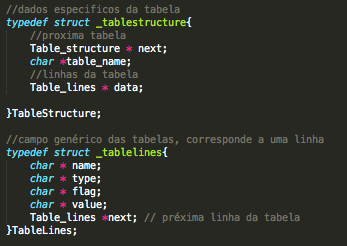
\includegraphics[scale=0.9]{table_structs.png}\\
Fig.10 - Estruturas das tabelas;
\end{center}

\indent A \textit{TableStructure} consiste num \textit{``header genérico''} que contém um ponteiro para a próxima tabela e um para outra estrutura \textit{TableLines} que representa cada linha da tabela.\\
\indent A estrutura \textit{TableLines} também tem um ponteiro para o próxima linha.

\newpage

\subsection{Criação de Tabelas}

\indent De seguida são apresentadas as funções responsáveis pela criação e manipulação de tabelas. No caso da \textit{create\_tables}, esta também insere os dados iniciais da \textbf{Outer Table} e da \textbf{Function Symbol Table}.

\begin{center}
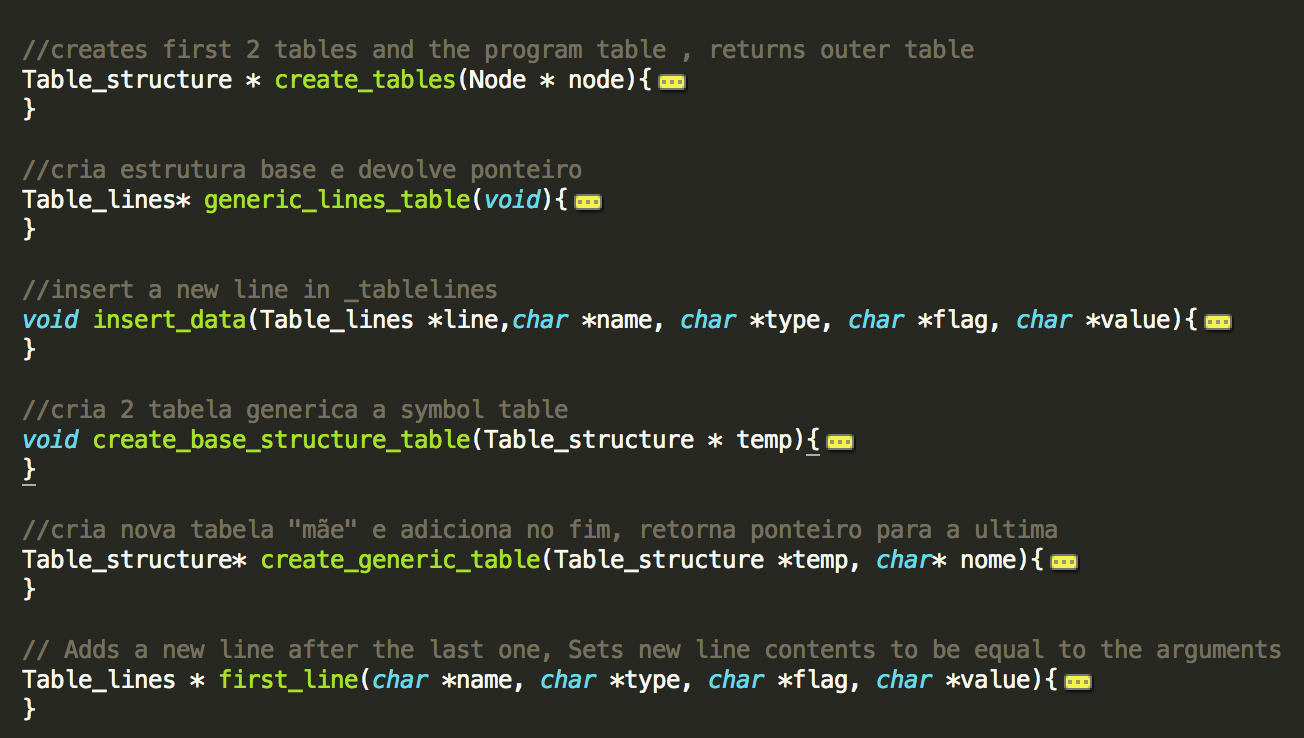
\includegraphics[scale=0.8]{table_functions.png}\\
Fig.11 - Funções de criação das tabelas;
\end{center}

\newpage

\subsection{Tratamento de erros}

\indent O tratamento de erros foi alterado na pós-meta, sendo que na meta normal quase nenhum erro foi tratado.\\
\indent Na fase de pós-meta foram adicionados os tratamentos de erros para símbolos duplicados, símbolos não definidos e sítios em que se espereva o identificador de tipo de variável.\\
\indent Embora o tratamento desses erros não tenha atingido a pontuação total, passámos de 205 pontos na meta 3 para 236 na pós-meta 3.\\

\begin{center}
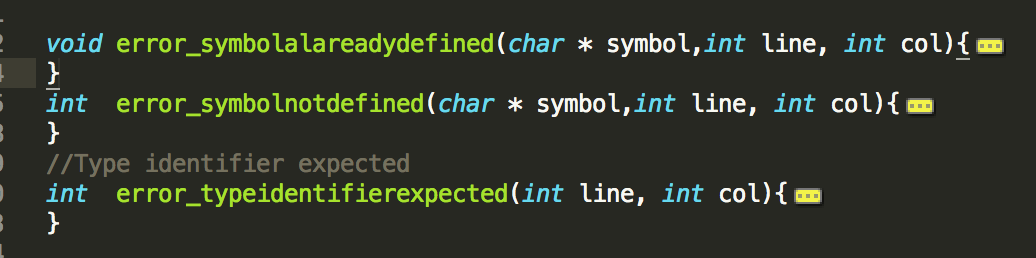
\includegraphics[scale=0.9]{errors.png}\\
Fig.12 - Funções de verificação de erros;
\end{center}

\newpage

\section{Geração de código}

\indent Na meta 4, não conseguimos obter qualquer ponto apesar do código produzido e várias tentativas.\\
\indent Conseguimos ainda assim colocar o programa a imprimir a declaração do \textit{printf} e a declaração das \textit{strings} necessárias para o \textit{writeln}.\\
\indent Para além da impressão das \textit{strings}, conseguimos ainda imprimir as variáveis dentro dos nós \textit{varDecl}.






\end{document}
